\section{Design}
\label{section:design}

In this section we describe the design of our classes and algorithms based on
the requirements established in \ref{section:requirements}.

\subsection{How to Run the Subsetter}

The success of the NetCDF Operators and similar tools demonstrate the need for
user-ready applications for the analyis of their data while the success of
tools such as CDAT validate the need for scriptability and customization of
basic and advanced operators.  We plan to provide both the scriptable
interface as well as a set of predefined tools.

The subsetter is the first in a series of parallel command-line tools based on
unstructured grids and the PGAS programming model.  It takes arguments
specifying specific variables (-v) or dimension ranges (-d) to extract, or at
a higher level a latitude and longitude bounding box (-b).  In this way it is
most akin to the NetCDF Operators' "kitchen sink" application.  Example usage
looks like:
\begin{itemize}
\item mpiexec -np 128 subsetter -b 20,-20,160,90 -v vorticity january.nc february.nc MJO\_vorticity\_janfeb.nc
\item mpiexec -np 64 subsetter -b 90,0,180,-180 -d levels,1,5 geopotential.nc
\end{itemize}

\subsection{Dataset Abstraction}

The subsetter minimally supports two forms of input file aggregation, either
across a specified dimension e.g. time or by taking the union of all input
files such that duplicate dimensions and variables within later files are
ignored.  These forms of aggregation are modeled after what is available when
using NetCDF Markup Language.\cite{NcML} NcML input is not directly supported
at this time but is planned for a future release. 

TODO

\subsection{Parallel IO Abstraction}

The use of Parallel NetCDF was selected because work on the HDF5/NetCDF4 was
incomplete at the time of development.

TODO

\subsection{The Global Arrays Library}

TODO PGAS

TODO ONE-SIDED COMMUNICATION

TODO GA DOES IT ALL

The subsetter was built using the GA library for the wealth of features it
provides which are tailored to our problem domain.  GA provides a distributed
dense multidimensional array programming abstraction and the data we will be
operating over is stored as dense arrays within NetCDF files.  It should be
noted that dense distributed arrays would also work well for regularly gridded
data.  However, due to the use of unstructured grid data, the algorithm for
subsetting the data will look quite different than for the structured case.
Recall that for unstructured grids, logically adjacent cells are not
necessarily adjacent in memory.  In order to evenly distribute a subset, a
single process will need to send a varying amount of data to any number of
other processes.  Certainly a collective operation could be considered, but GA
provides the necessary functionality without needing any explicit cooperation
from any other process.  Any given process will simply put the section of the
subset into the remote process's memory.  It is unclear how point-to-point
communications could mimic the ease of use of the interface provided by GA's
one-sided operations.

Each dimension of the data has two arrays associated with it, a bitmask and an
integer array representing the new indices of the dimension in case of a
subset.  For instance, if any of the bits are turned off, the corresponding
index array will have negative values.  The remaining values of the index
array will increase monotonically, skipping the negative or masked indices.
The bitmasks are generated based on a rectangular latitude and longitude
region specified on the command-line, or by specifying one or more indices of
a dimension to select.  Although a rectangular region is currently used for
simplicity, once translated the bitmasks allow for arbitrary subsets to be
defined.  These bitmasks are then used to evenly distribute the resultant
subset across all processes.  Note that these bitmask and associated index
arrays are one-dimensional and distributed.

REMOVE
There are certain GA operations which are tailored for use on one-dimensional
arrays such as the bitmasks.  These operations include \verb=GA_Patch_enum=,
\verb=GA_Scan_add=, \verb=GA_Scan_copy=, \verb=GA_Pack=, and \verb=GA_Unpack=.
The remaining GA operations are N-dimensional and one-sided and include
\verb=NGA_Scatter=, \verb=NGA_Gather=, \verb=GA_Put=...
REMOVE

The vast majority of functionality within the subsetter is provided by either
PnetCDF or GA.  GA allocates and evenly distributes the arrays which are then
filled with data by PnetCDF.  GA operations are then used to prepare the data
for packing at which point a custom n-dimensional packing routine is used.
The packed, evenly-distributed data is then written back to disk using
PnetCDF.  Of these algorithms, the novel ones include reindexing the masks,
reindexing the connectivity variables, and the n-dimensional pack routine.

\subsection{The Algorithms}

The one-sided communications and PGAS model afforded by GA allowed us to
develop some novel algorithms for the manipulation of unstructured grids.  In
this section we diagram and describe the algorithms we developed.

\subsubsection{Partial Sum}

\begin{figure}[!t]
\center
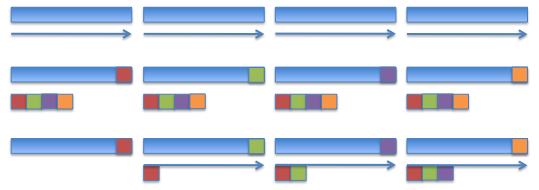
\includegraphics[width=3.5in]{images/partialsum}
\caption{Distributed partial sum on a 1-D array}
\label{fig:partialsum}
\end{figure}

\subsubsection{REINDEXING OF DISTRIBUTED MASKS}

Creating the index array associated with a mask is the easiest of the
algorithms.  It only requires three specific GA operations, \verb=GA_Fill=,
\verb=GA_Patch_enum= and \verb=GA_Unpack=.  \verb=GA_Fill= fills the index
array with a value of $-1$.  \verb=GA_Patch_enum= enumerates the values of a
second array starting from zero with an increment of 1.  \verb=GA_Unpack=
expands the enumerated array values into the filled array based on the
associated mask array.

\subsubsection{REINDEXING OF CONNECTIVITY VARIABLES}

Recall that the connectivity variables are those which map from one index to
one or more other indices such as from a cell index to each of its corner
indices.  A typical subset operation reduces the number of cells, corners, and
edges within the data, so it is important to maintain the integrity of these
mapping arrays such that they map to real indices.

The reindexing of the connectivity variables relies on the recalculated index
array of the associated domain.  For example, when reindexing the mapping from
cells to corners, the recalculated corners index array is required.  The
mapping values represent indices into the recalculated index array, so the
values are organized into set of indices for the GA routine \verb=NGA_Gather=
to query.  The \verb=NGA_Gather= routine gathers array elements from a global
array into a local array and in this case gathers the new values for the
mapping.  The gathered values then appropriately replace the old mapping
values.

\subsubsection{N-DIMENSIONAL PACK ROUTINE}

TODO -- Consider pseudo code?  \verb=GA_Scan_add= routine was used to perform
partial sums on all masks. That helps determine where to \verb=NGA_Put= the
subset data.

